\documentclass[12pt,a4paper]{book}

% Formato del documento
%\usepackage[papersize={210mm,297mm},inner=3.5cm,outer=2cm,top=2.5cm,bottom=2.5cm]{geometry}
%\renewcommand{\baselinestretch}{1}
%\setlength{\parskip}{8pt}

\usepackage[utf8]{inputenc}
\usepackage{amssymb}
\usepackage{amsmath}
\usepackage{graphicx}
\usepackage{tikz}
\usepackage{tkz-graph}
\usepackage{hyperref}
\usepackage[parfill]{parskip}
\usepackage{float}
\renewcommand{\chaptername}{Capítulo}
\renewcommand{\contentsname}{Índice}
\renewcommand{\bibname}{Bibliografía}
\renewcommand{\figurename}{Figura}

\definecolor{verde_oscuro}{rgb}{0.0, 0.5, 0.0}

\newtheorem{defi}{Definición}[section]
\newtheorem{prop}{Proposición}[section]
\newtheorem{propi}{Propiedades}[section]
\newtheorem{lema}{Lema}[section]
\newtheorem{tma}{Teorema}[section]
\newtheorem{cor}{Corolario}[section]
\newtheorem{nota}{Nota}[section]
\newtheorem{ejem}{Ejemplo}[section]

\hypersetup{
    colorlinks=true,
    linkcolor=blue,
    filecolor=magenta,      
    urlcolor=cyan,
    pdftitle={Overleaf Example},
    pdfpagemode=FullScreen,
    }

\urlstyle{same}

%%%%%%%ALTERNATIVA 2%%%%%%%%%%%%
\textheight=21cm
\textwidth=17cm
%\topmargin=-1cm
\oddsidemargin=0cm
\evensidemargin=0cm
\parindent=0mm
\pagestyle{plain}
%%%%%%%%%%%%%%%%%%%%%

%%%%%%%  Comando Portada  %%%%%%%%%%%
% Ajustes de geometría si la portada sigue sin caber
% \geometry{a4paper, top=1cm, bottom=1cm, left=1cm, right=1cm} 

\newcommand{\nuevaportada}[6]{
    \thispagestyle{empty}
    \begin{center}
        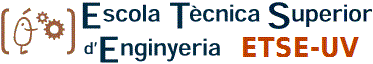
\includegraphics[width=0.5\textwidth]{images/logo.png}
        
        \vspace{0.3cm} % Espacio reducido
        {\Large\bfseries\textsc{M\'aster Universitario en #1}\par}
        
        \vspace{0.3cm} % Espacio reducido
        
\includegraphics[width=0.4\textwidth]{images/uv.png}
        
        \vspace{0.3cm} % Espacio reducido
        {\Large\bfseries\textsc{Trabajo de Fin de M\'aster}\par}
        
        \vspace{0.5cm} % Mantener este espacio un poco más grande para el título
        {\Large\bfseries #2\par}
        
        \vspace{1.5cm} % Reducido a 1.5cm desde 2cm
        \begin{flushright}
            \begin{tabular}{l} 
                {\large\bfseries\textsc{Autor:}} \\
                {\large\textsc{#3}} \\ [0.3cm] % Espacio reducido
                {\large\bfseries\textsc{Tutora:}} \\ 
                {\large\textsc{#4}} \\ [0.3cm] % Espacio reducido
                {\large\bfseries #5} 
            \end{tabular}
        \end{flushright}
    \end{center}
    % Eliminamos \clearpage de aquí, ya que la portada debe ser una sola página
    % Si necesitas un salto de página después de la portada, lo añades en el documento principal.
}

\begin{document}

\nuevaportada{Ciencia de Datos}{Problema de Localización de Centros k-Balanceado Multiobjetivo}{Manuel Rubio Martínez}{Anna Martínez Gavara}{Abril, 2025}

\clearpage

\newpage
\tableofcontents

\newpage

\section*{Resumen}
Aquí va el contenido de tu resumen en español. Explica brevemente el objetivo, la metodología, los resultados y las conclusiones de tu TFM.

\newpage

\section*{Abstract}
Here goes the content of your abstract in English. Briefly explain the objective, methodology, results, and conclusions of your TFM.

\newpage

\section*{Resum}
Aquí va el contingut del teu resum en valencià. Explica breument l'objectiu, la metodologia, els resultats i les conclusions del teu TFM.

\newpage

\chapter{Preliminares}
\section{Introducción}
\begin{defi}[Dominio de una función]
Dada una función $f: X \to Y$, su \textbf{dominio} es el conjunto de todos los valores de entrada para los cuales la función está definida. En este caso, el dominio es $X$.
\end{defi}

\begin{defi}[Imagen de una función]
Dada una función $f: X \to Y$, su \textbf{imagen} es el subconjunto formado por todos los valores que la función toma realmente. Se denota como $\text{Im}(f)$ o $f(X)$, y se define como:
$$ f(X) = \{y \in Y \mid \exists x \in X, f(x) = y \} $$
\end{defi}

\begin{defi}[Conjunto convexo]
Un conjunto $C \subseteq \mathbb{R}^n$ es \textbf{convexo} si para cualquier par de puntos $x, y \in C$, el segmento de recta que los une está completamente contenido en $C$. Formalmente, para todo $x, y \in C$ y para todo $\lambda \in [0, 1]$:
$$ \lambda x + (1-\lambda)y \in C $$
\end{defi}

\begin{defi}[Función lineal]
Una función $f: \mathbb{R}^n \to \mathbb{R}^m$ es \textbf{lineal} si satisface dos propiedades: aditividad y homogeneidad. Es decir, para cualesquiera vectores $\mathbf{x}, \mathbf{y} \in \mathbb{R}^n$ y cualquier escalar $\alpha \in \mathbb{R}$:
\begin{enumerate}
    \item $f(\mathbf{x}+\mathbf{y}) = f(\mathbf{x}) + f(\mathbf{y})$ (Aditividad)
    \item $f(\alpha \mathbf{x}) = \alpha f(\mathbf{x})$ (Homogeneidad de grado 1)
\end{enumerate}
\end{defi}

\begin{defi}[Función continua]
Intuitivamente, una función $f$ es continua si cambios pequeños en la entrada provocan cambios pequeños en la salida (no hay saltos abruptos). Formalmente, una función $f: X \to Y$ es continua en un punto $c \in X$ si para todo $\epsilon > 0$, existe un $\delta > 0$ tal que si la distancia de $x$ a $c$ es menor que $\delta$, entonces la distancia de $f(x)$ a $f(c)$ es menor que $\epsilon$.
$$ \forall \epsilon > 0, \exists \delta > 0 : |x-c| < \delta \implies |f(x)-f(c)| < \epsilon $$
La función es continua en su dominio si es continua en todos sus puntos.
\end{defi}

\begin{defi}[Función diferenciable]
Una función real de una variable real $f: \mathbb{R} \to \mathbb{R}$ es \textbf{diferenciable} en un punto $x_0$ de su dominio si su derivada existe en ese punto. Esto significa que la función puede ser aproximada localmente por una función lineal (su recta tangente) en el entorno de $x_0$. Formalmente, si el siguiente límite existe:
$$ f'(x_0) = \lim_{h \to 0} \frac{f(x_0+h) - f(x_0)}{h} $$
Para funciones de varias variables, $f: \mathbb{R}^n \to \mathbb{R}^m$, la diferenciabilidad implica la existencia de una transformación lineal  que aproxima el comportamiento de la función en un punto.
\end{defi}

\begin{defi}[Conjunto numerable]
Un conjunto es \textbf{numerable} (o contable) si existe una correspondencia uno a uno entre los elementos del conjunto y un subconjunto de los números naturales $\mathbb{N} = \{1, 2, 3, \dots\}$. Esto significa que se puede crear una lista (finita o infinita) que contenga todos los elementos del conjunto. El conjunto de los números enteros $\mathbb{Z}$ y el de los números racionales $\mathbb{Q}$ son numerables, mientras que el conjunto de los números reales $\mathbb{R}$ no lo es.
\end{defi}
\section{Modelo Matemático}

\begin{defi}
Un algoritmo \textbf{"greedy"} (codicioso) es un método construcción de soluciones para un problema de optimización,
de manera que en cada paso se escoge la mejor posible, aunque esto no lleve finalmente a un óptimo global.
\end{defi}

\bigskip

\begin{defi}
Un algoritmo \textbf{"greedy randomizado"} se basa en el "greedy", pero en cada paso se elige de forma aleatoria entre un conjunto de mejores opciones.
Si el conjunto de opciones es el total, el algoritmo es "random".
\end{defi}

\chapter{Introducción}
La optimización es una de las ramas fundamentales dentro de las matemáticas aplicadas. Se utiliza tanto en economía como en ingeniería informática o ciencias naturales y sociales.

En esencia, la optimización trata de encontrar la mejor solución posible a un problema.

Un problema de optimización se compone de tres elementos clave:
\begin{itemize}
    \item \textbf{Variables de decisión:} Las carreteras a tomar en una ruta, el número de personas a contratar para un trabajo o las ubicaciones en las que construir una instalación.
    \item \textbf{Función objetivo:} El criterio que se desea optimizar, ya sea para minimizar (costes, tiempos de producción, distancias) o para maximizar (eficacia de anuncios publicitarios, beneficios o la supervivencia en tratamientos médicos).
    \item \textbf{Restricciones del problema:} Límite de carga de camiones, un presupuesto máximo a gastar, limitaciones de maquinaria o de personal, etcétera.
\end{itemize}

Para abordar estos problemas de manera sistemática y eficiente, la optimización a menudo implica una formulación matemática que simplifica las variables del caso real en un plano abstracto donde es más práctico resolverlos. 

\section{Historia de la optimización}
El origen de la optimización se remonta a la antigua Grecia, donde matemáticos como Euclides y Arquímedes la utilizaban para buscar soluciones a problemas en el área de la geometría.

La versión que conocemos hoy en día no empezó a desarrollarse hasta el siglo XVII, con el desarrollo del cálculo diferencial por parte de Isaac Newton y Gottfried Wilhelm Leibniz, con el que se empezaron a estudiar las funciones y sus puntos extremos,
donde se encontraban sus máximos y mínimos.

No hubo grandes avances hasta mediados del siglo XX, cuando, fruto de la necesidad de resolver problemas logísticos durante la Segunda Guerra Mundial, se desarrolló la programación lineal (creada por el matemático George Dantzig),
que sentó las bases para el posterior surgimiento de la programación no lineal, programación entera y programación dinámica.

A pesar de todos estos avances, la mayoría de problemas del mundo real, especialmente aquellos que dependen de un gran número de variables, con funciones objetivo complejas y restricciones no lineales,
acaban siendo demasiado complejos computacionalmente para tratar de buscar su solución exacta, lo que propició el surgimiento de los metaheurísticos.

Los algoritmos metaheurísticos (que explicaremos en profundidad más adelante) sientan las bases de la optimización moderna, que se centra en la búsqueda de soluciones aproximadas, pero próximas al óptimo, en un tiempo de procesamiento aceptable.

Para la ciencia de datos serán cruciales para el desarrollo de algoritmos en diversos ámbitos:
\begin{itemize}
    \item \textbf{Clustering:} El algoritmo \textbf{k-means} particiona el espacio de observaciones en un número determinado de clústeres (grupos) y determina qué observaciones pertenecen a cada uno de ellos. 
    Si intentásemos encontrar la solución exacta, sería computacionalmente muy costoso, y la naturaleza del algoritmo hace que la solución sea dependiente de los grupos iniciales (generados aleatoriamente), pudiendo caer en óptimos locales.
    Las metaheurísticas ayudan a solventar estos problemas.
    
    \item \textbf{Selección de variables:} En la construcción de modelos de predicción, solemos encontrarnos con una gran cantidad de variables, por lo que definir el modelo con base en todas ellas no es factible. Mediante metaheurísticos podemos 
    reducir significativamente la dimensión del espacio, utilizando un subespacio con las variables que mejor sirvan al modelo.
    
    \item \textbf{Ajuste de hiperparámetros:} Modelos de inteligencia artificial como las redes neuronales necesitan ajustar sus hiperparámetros para ser eficaces. Esto también es un problema de optimización, donde los metaheurísticos pueden superar la típica \textit{búsqueda en cuadrícula} (\textit{grid search}) de parámetros.
\end{itemize}

\color{red} citar a Libros de texto sobre optimización y algoritmos heurísticos: Por ejemplo, "Metaheuristics: From Design to Implementation" de E.K. Burke y G. Kendall, o "Introduction to Optimization" de E.J. Anderson. \color{black}

\section{Formulación Matemática}

Para expresar un problema de optimización de forma matemática, definimos las tres partes en las que se puede descomponer:

\begin{itemize}
    \item \textbf{Variables de Decisión:} Las incógnitas del problema. Son los valores que deberemos modificar para obtener la solución o soluciones óptimas. Se representan como un vector $\mathbf{x} = (x_1, x_2, \ldots, x_n)$, donde $n$ es el número de variables.

    \item \textbf{Función Objetivo:} Función que se desea minimizar o maximizar. Se denota comúnmente como $f(\mathbf{x})$, donde $f$ es la función que establece la relación entre las variables ($\mathbf{x}$) y el objetivo que deseamos optimizar.
    Por ejemplo:
    $$ \min_{\mathbf{x}} f(\mathbf{x}) \quad \text{o} \quad \max_{\mathbf{x}} f(\mathbf{x}) $$
    La función $f: \mathbb{R}^n \to \mathbb{R}$ mapea el vector de variables a un valor escalar, el cual buscaremos mejorar.

    \item \textbf{Restricciones:} Son las condiciones o limitaciones que deben satisfacer las variables de decisión. Pueden ser de igualdad o de desigualdad. Se expresan generalmente como:
    \begin{align*}
        g_i(\mathbf{x}) &\le 0 & \quad \text{para } i = 1, \ldots, m \\
        h_j(\mathbf{x}) &= 0 & \quad \text{para } j = 1, \ldots, p
    \end{align*}
    Donde $g_i(\mathbf{x})$ son las $m$ restricciones de desigualdad y $h_j(\mathbf{x})$ son las $p$ restricciones de igualdad.
    En caso de tener restricciones del tipo $g_k(\mathbf{x})\geq0$, se puede transformar a $\leq$ sabiendo que $-g_k(\mathbf{x}) \leq 0$.
    
    Además de restricciones funcionales, también pueden existir restricciones sobre el dominio de las variables, como $x_k \ge 0$ (variables no negativas) o $x_k \in \{0,1\}$ (variables binarias).
\end{itemize}

Ahora sí, pasadas las definiciones previas, un problema completo de optimización se formula de la siguiente manera:
$$
\begin{array}{ll}
\text{Minimizar (o Maximizar)} & f(\mathbf{x}) \\ \\
\text{Sujeto a:} & g_i(\mathbf{x}) \le 0, \quad i = 1, \ldots, m \\
& h_j(\mathbf{x}) = 0, \quad j = 1, \ldots, p \\
& \mathbf{x} \in X
\end{array}
$$
Donde $X$ representa el conjunto de factibilidad o dominio de las variables de decisión.

\subsection{Tipos de Óptimos: Global vs. Local}

En optimización, es fundamental distinguir entre los distintos tipos de soluciones óptimas, ya que la función objetivo puede tener múltiples puntos donde alcance valores extremos. Por eso hay que diferenciar entre los óptimos locales y globales.

\subsubsection{Óptimo Global}
Un óptimo global es el mejor valor posible que, dentro del dominio de factibilidad $\mathbf{X}$, puede tomar la función objetivo. Esto significa que no existe ninguna otra solución que ofrezca un valor estrictamente mejor que el del óptimo global.

Es la solución que siempre querremos obtener al resolver un problema de optimización.

Si estamos minimizando $f(\mathbf{x})$, el punto $\mathbf{x}^* \in \mathbf{X}$ es un óptimo global si
$$f(\mathbf{x}^*)\leq f(\mathbf{x}) \quad \forall \mathbf{x}\in X$$

\subsubsection{Óptimo Local}
Un óptimo local es un punto donde la función objetivo alcanza el mejor valor posible dentro de una región próxima, pero no necesariamente en todo el dominio. Pueden existir infinidad de óptimos locales.

Si estamos minimizando $f(\mathbf{x})$, el punto $\mathbf{x}^* \in \mathbf{X}$ es un óptimo local si existe un $\epsilon>0$ tal que
$$f(\mathbf{x}^*)\leq f(\mathbf{x}) \quad \forall \mathbf{x}\in X \text{ que cumpla que }||\mathbf{x}-\mathbf{x}^*||<\epsilon$$
Donde $||\cdot||$ denota una métrica de distancia.

Un par de ejemplos para distinguir los dos tipos de óptimos:
\begin{itemize}
    \item Si consideramos la elevación de la superficie terrestre como la función objetivo a maximizar, un \textbf{óptimo local} será la cima de cualquier montaña. Es el punto más alto si consideramos como entorno próximo la \textbf{propia} montaña.
    \item En contraste, el \textbf{óptimo global} sería la cima del Monte Everest, el punto más alto de toda la geografía terrestre.
\end{itemize}

\subsection{Optimización Lineal vs. No Lineal}

Otra parte importante a tener en cuenta en los problemas de optimización es la forma de sus funciones, tanto de la objetivo como de las restricciones. Esto determinará si el problema puede ser resuelto fácilmente de manera exacta o si requerirá de métodos más complejos con soluciones aproximadas.

\subsubsection{Optimización Lineal}
Diremos que un problema es de \textbf{optimización lineal} cuando tanto la función objetivo como todas las funciones de las restricciones son lineales (con respecto a las variables de decisión). 

Características principales:
\begin{itemize}
    \item La función objetivo tiene la forma $f(\mathbf{x})=c_1x_1+c_2x_2+...+c_nx_n$ con los $c_i \in \mathbb{R} \quad \forall i \in 1,2,...,n$.
    \item Todas las restricciones son lineales, con la forma $a_1x_1+a_2x_2+...+a_nx_n\leq b$ o $=b$.
    \item Estas condiciones hacen que el conjunto de soluciones factibles ($X$) tenga la forma de un poliedro convexo, lo que simplifica la búsqueda del óptimo.
    \item El algoritmo Simplex, explicado en detalle en \cite{Dantzig1951}, es el más extendido para resolver este tipo de problemas y garantiza encontrar el óptimo global, si existe.
\end{itemize}

\subsubsection{Optimización No Lineal}
Diremos que un problema es de \textbf{optimización no lineal} cuando al menos una de sus funciones (objetivo o de restricción) es no lineal (con respecto a sus variables de decisión). 

Características principales:
\begin{itemize}
    \item La función objetivo $f(\mathbf{x})$ o alguna de sus restricciones $g_i(\mathbf{x})$ o $h_j(\mathbf{x})$ contiene términos no lineales. Por ejemplo:
    $$f(\mathbf{x})=2x_1^2+5x_2^7-\ln(x)$$
    \item El conjunto de soluciones factibles puede ser no convexo, lo que deriva en múltiples óptimos locales y en una extrema complejidad a la hora de buscar el óptimo global.
    \item La mayoría de algoritmos para resolverlos suelen utilizar técnicas de búsqueda local y no garantizan encontrar el óptimo global.
\end{itemize}

Ejemplos:
\begin{itemize}
    \item \textbf{Lineal:} Una fábrica busca maximizar su beneficio produciendo varios artículos, donde cada uno consume una cantidad fija de recursos (horas de máquina, materia prima) y genera un beneficio fijo, con restricciones de recursos y uso de las máquinas.
    \item \textbf{No lineal:} Encontrar los parámetros de una curva que se ajustan a unos datos concretos, minimizando el error cuadrático medio entre la aproximación (la curva) y el valor exacto de los datos.
\end{itemize}

\subsection{Optimización Discreta vs. Continua}
Probablemente, la mayor distinción en cuanto a problemas de optimización la veamos en base a la naturaleza de sus variables de decisión. Que sean continuas o discretas
limitará en gran medida el tipo de algoritmos que puedan utilizarse para resolverlos.

\subsubsection{Optimización Continua}
En la optimización continua, las variables de decisión pueden tomar cualquier valor real dentro de su dominio o rango permitido. Es decir, no están restringidas a tomar valores enteros, a un conjunto finito o a un conjunto numerable de posibles soluciones. Esto las hace adecuadas para modelar fenómenos que varían de forma suave, como el tiempo, el espacio, la temperatura, etcétera.

Características principales:
\begin{itemize}
    \item Variables pertenecientes a un espacio continuo, típicamente $\mathbb{R}^n$.
    \item Las funciones objetivo $f(\mathbf{x})$ y sus restricciones $g_i(\mathbf{x}), \;h_j(\mathbf{x})$ suelen ser continuas y diferenciables.
    \item Las técnicas de resolución a menudo involucran cálculo diferencial para encontrar el mejor camino de mejora de la solución.
\end{itemize}

\subsubsection{Optimización Discreta}
En este caso, las variables de decisión están restringidas a tomar valores de un conjunto finito o, al menos, numerable. Los casos más comunes son variables restringidas a tomar valores enteros (0,1,2...), binarios (0,1) o variables que representan la elección de elementos de un conjunto específico (por ejemplo, el "trabajador 1" o el "trabajador 2").

Características principales:
\begin{itemize}
    \item Las variables pertenecen al espacio discreto.
    \item No se pueden utilizar directamente las técnicas de cálculo diferencial que, en cambio, sí se podrían usar en el espacio continuo.
    \item Los problemas suelen ser más complejos de resolver y computacionalmente más costosos, por lo que suelen requerir algoritmos específicos como la programación entera, la programación dinámica o métodos combinatorios para poder resolverlos.
\end{itemize}

Ejemplos:
\begin{itemize}
    \item Como casos continuos, tenemos el diseño de la aerodinámica de un avión (se modelan los parámetros de las curvas de la superficie) o la velocidad óptima de un vehículo para reducir su consumo de combustible.
    \item Como casos discretos, tenemos el problema de la mochila (escoger el mayor valor en elementos de un conjunto sin exceder una capacidad dada) o la planificación de rutas.
\end{itemize}

Para estas primeras partes introductorias he tomado como referencia el libro \cite{Numerical_optimization_nocedal_wright} de Numerical Optimization de Jorge Nocedal y Stephen J. Wright.

\section{Optimización Combinatoria}
La optimización combinatoria es la rama de la optimización y las matemáticas aplicadas que se centra en encontrar una solución óptima dentro de un conjunto de soluciones finito o numerable. Aunque la cantidad de posibles soluciones pueda ser finita, esto no implica que el problema sea sencillo. De hecho, la gran mayoría de los problemas de optimización combinatoria pertenecen a la clase de complejidad NP-difícil.

La naturaleza NP-difícil de estos problemas implica que el tiempo necesario para encontrar la solución óptima crece de manera exponencial a medida que aumenta el tamaño del problema. Esto hace que la búsqueda exhaustiva de la solución sea computacionalmente inviable para la mayoría de los casos de estudio del mundo real.

\textbf{Características principales:}
\begin{itemize}
    \item \textbf{Espacio de soluciones discreto:} Las variables de decisión están restringidas a un conjunto finito o numerable de valores, como la selección o no de un elemento, o la ordenación de un conjunto (están dentro de los casos de \textbf{optimización discreta}). 
    \item \textbf{Complejidad computacional elevada:} A menudo, el número de soluciones posibles es astronómicamente grande, lo que requiere algoritmos especializados para explorar el espacio de búsqueda de manera eficiente.
    \item \textbf{Estructura del problema:} Las técnicas de resolución aprovechan la estructura combinatoria subyacente del problema, utilizando métodos como la programación entera, la teoría de grafos o los algoritmos metaheurísticos.
\end{itemize}

Un ejemplo fundamental, que además es la base del problema que se tratará en este TFM, es la \textbf{selección de un subconjunto}. El objetivo es encontrar, en un conjunto de $n$ elementos, un subconjunto de tamaño $k$ que optimice (minimice o maximice) una o varias funciones objetivo. El número total de subconjuntos posibles viene dado por el coeficiente binomial:

$$
    \binom{n}{k} = \frac{n!}{(n-k)!k!}
$$

Para ilustrar la explosión combinatoria, consideremos un caso sencillo, con $n=50$ y $k=5$. El número de combinaciones posibles es:

$$
    \binom{50}{5} = \frac{50!}{(50-5)!5!} = 2,118,760
$$

Si escalamos el problema a dimensiones más realistas, como $n=5000$ y $k=50$, la cantidad de soluciones posibles se dispara a una cifra del orden de $2.28 \times 10^{120}$. Evaluar cada una de estas soluciones para encontrar la óptima de forma exacta es una tarea imposible, incluso para los superordenadores más potentes, ya que requeriría tiempos de computación demasiado elevados.

Otros ejemplos clásicos de optimización combinatoria incluyen el \textbf{Problema del Viajante de Comercio (TSP)}, que busca la ruta más corta que visita un conjunto de ciudades una sola vez; el \textbf{problema de la mochila}, que consiste en seleccionar los objetos más valiosos sin superar una capacidad de peso; o la \textbf{planificación de horarios}, donde se asignan recursos (como aulas o profesores) a franjas horarias para satisfacer un conjunto de restricciones.

\section{Optimización Multiobjetivo}
A diferencia de la optimización típica mono-objetivo, donde se busca optimizar una única función, la optimización multiobjetivo aborda problemas en los que es necesario mejorar simultáneamente dos o más funciones objetivo que, a menudo, están en conflicto entre sí. Mejorar una suele implicar el empeoramiento de la otra. Por ejemplo, en el diseño de un vehículo, minimizar el consumo de combustible (objetivo 1) puede estar en conflicto con maximizar la potencia del motor (objetivo 2).

La principal ventaja de la optimización multiobjetivo respecto a la mono-objetivo radica en poder reflejar la complejidad de las decisiones en el mundo real.
Permite analizar las compensaciones (\textit{trade-offs}) de forma explícita, cuantificando cuánto se debe sacrificar de un objetivo para conseguir una mejora en otro.\\
Al ofrecer un espectro de soluciones óptimas y equilibradas, en lugar de una única respuesta, facilita la toma de decisiones más realistas con una mejor estrategia.

Aquí radica la diferencia fundamental con la optimización mono-objetivo. No existe el concepto de "solución óptima" única. Raramente existe una solución que sea la mejor para todos los objetivos a la vez. En su lugar, lo que se busca es encontrar un conjunto de soluciones que representen las mejores compensaciones posibles.

Este conjunto de soluciones se conoce como \textbf{Frente de Pareto}. 
Una solución es \textbf{no dominada} (u óptima en el sentido de Pareto) si no existe otra solución factible que la mejore en al menos un objetivo sin empeorar en ninguno de los demás.

\begin{figure}[H]
    \centering
    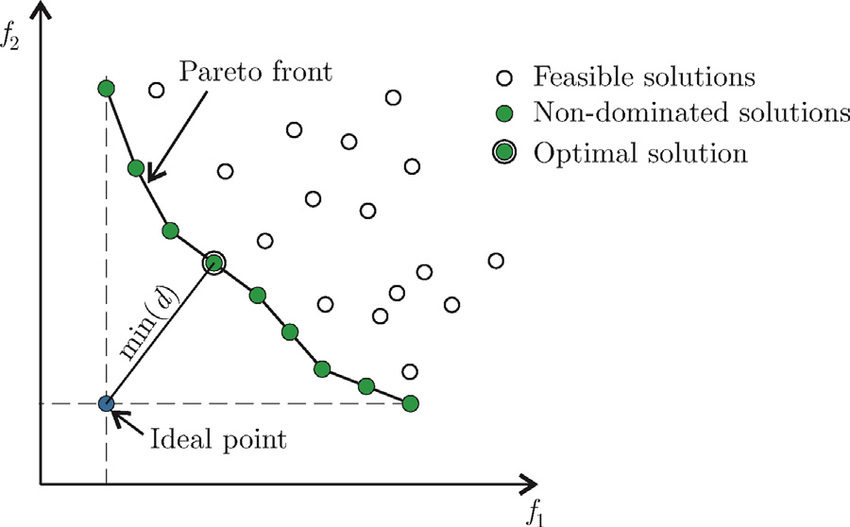
\includegraphics[width=0.6\textwidth]{images/pareto_front.png}
    \caption{Ilustración de un Frente de Pareto para un problema de minimización con dos objetivos ($f_1, f_2$). Las soluciones en verde son óptimas y pertenecen al Frente de Pareto, ya que no se puede mejorar un objetivo sin empeorar el otro. El punto ideal, que estaría en la parte inferior izquierda de la gráfica, sería la mejor solución imaginable combinando lo mejor de todas las soluciones. Las soluciones sin colorear están dominadas por alguna de las verdes\cite{Bre2017}.}
    \label{fig:pareto}
\end{figure}

\subsection{Métodos Exactos}

Los métodos exactos para la optimización multiobjetivo tienen como finalidad encontrar el Frente de Pareto al completo. Sin embargo, al igual que en sus contrapartes mono-objetivo, se enfrentan al mismo obstáculo: la complejidad computacional. La mayoría de estos problemas son \textbf{NP-hard}.

No obstante, para problemas sencillos, con pocas variables y reducido espacio de soluciones, se pueden resolver con los siguientes métodos:

\begin{itemize}
    \item \textbf{Métodos de Ponderación (Weighted Sum):} Transforman el problema multiobjetivo en problemas mono-objetivo, asignando pesos a cada una de las funciones objetivo y sumándolos para crear una única función agregada. Al variar sistemáticamente los pesos, se pueden ir generando las soluciones del Frente de Pareto. Sin embargo, este método no garantiza encontrar todas las soluciones si el frente tiene una forma no convexa.

    \item \textbf{Método de las Restricciones Épsilon ($\epsilon$-constraint):} Consiste en optimizar una de las funciones objetivo, convirtiendo el resto en restricciones que limitan su valor a un máximo $\epsilon$.\\
    Modificando los valores de $\epsilon$ para cada objetivo-restricción, se puede explorar y reconstruir el Frente de Pareto. A diferencia del método de ponderación, este sí puede encontrar soluciones en frentes no convexos.

    \item \textbf{Algoritmos de Ramificación y Acotación (Branch and Bound) Multiobjetivo:} Estos algoritmos extienden el clásico \textit{Branch and Bound}. El proceso de ramificación es similar (se divide el problema en subproblemas más pequeños), pero la fase de acotación (o poda) es más compleja. En lugar de usar una única cota, se trabaja con conjuntos de cotas (un vector por cada objetivo). Una rama del árbol de búsqueda se poda solo si se puede demostrar que no puede contener ninguna solución no dominada en comparación con las soluciones ya encontradas.

    \item \textbf{Algoritmos de Ramificación y Corte (Branch and Cut) Multiobjetivo:} De manera análoga, esta técnica extiende \textit{Branch and Cut}. Se añaden planos de corte (restricciones adicionales) no solo para mejorar la relajación del problema mono-objetivo, sino para refinar la aproximación del espacio de soluciones factibles en el dominio multiobjetivo, permitiendo podar ramas del árbol de búsqueda de forma más eficiente.
\end{itemize}


\subsection{Metaheurísticos}
Las metaheurísticas aparecen con el desarrollo de las ciencias de la computación como principal solución a estos problemas. Allí donde los métodos exactos no serían capaces de encontrar el óptimo,
los metaheurísticos buscan soluciones "buenas" en tiempos de ejecución razonables, sacrificando la garantía de optimalidad global que proporcionan los métodos exactos.

Generalmente combinan heurísticas con aleatoriedad para obtener soluciones de calidad, a la vez que se explora el espacio buscando nuevos óptimos locales.\\
Estos métodos combinan dos estrategias:
\begin{itemize}
    \item \textbf{Exploración:} Capacidad de recorrer diversas áreas del espacio de búsqueda para encontrar nuevas soluciones, evitando quedar atrapado en óptimos locales.
    \item \textbf{Explotación:} Capacidad de intensificar la búsqueda en una región prometedora para encontrar los mejores óptimos locales dentro de ella.
\end{itemize}

Son algoritmos muy generales, fáciles de implementar y adaptables a casi 
cualquier problema de optimización. Las principales metaheurísticas son:
\begin{itemize}
    \item \textbf{Algoritmos Genéticos (GA - Genetic Algorithms)}\\
    Inspirados en la selección natural y la genética, se basan en la generación aleatoria de soluciones y en el cruce de las más prometedoras entre sí, 
    mientras se añaden mutaciones (pequeñas modificaciones en las soluciones) para aportar diversidad.
    
    \item \textbf{Recocido Simulado (SA - Simulated Annealing)}\\
    Basado en un proceso físico, simula el recocido de metales (calentarlos y enfriarlos para alterar su estructura). Explora soluciones aceptando movimientos de mejora, pero también aquellos que puedan empeorar la solución, 
    en función de una probabilidad dependiente de una variable "temperatura", que decrece con el paso de las iteraciones. En fases tempranas, una temperatura alta favorece la exploración, mientras que en fases finales una temperatura baja favorece la explotación.
    
    \item \textbf{Búsqueda Tabú (TS - Tabu Search)}\\
    Genera una lista `tabú` que actúa como memoria a corto plazo del algoritmo, incluyendo los movimientos recientes con el objetivo de no repetir soluciones y así forzar la exploración de nuevas zonas, aunque eso conlleve aceptar movimientos que no sean los mejores posibles.
    
    \item \textbf{Optimización por Colonia de Hormigas (ACO - Ant Colony Optimization)}\\
    Diseñado originalmente para problemas de rutas, construye soluciones iterativamente a través de un grafo, cuyas aristas se van ponderando a medida que se generan soluciones de calidad.
    
    \item \textbf{GRASP (Greedy Randomized Adaptive Search Procedure)}\\
    Algoritmo fundamentado en dos fases. Una primera de construcción, en la que se genera una solución mediante un proceso aleatorizado, y una segunda de búsqueda local, en la que se intenta mejorar la solución generada.
\end{itemize}

\section{Motivación para la Ciencia de Datos}

\color{red}
Motivación para ciencia de dato Por qué los métodos clásicos no siempre sirven, cómo se combina con técnicas de aprendizaje (refuerzo), visión interdisciplinar: matemática, computacional, aplicada.

No entiendo esta parte, he introducido la parte del uso de optimización en ciencia de datos antes, esto debe ser por qué yo, habiendo hecho el máster de ciencia de datos, he escogido un tfm de optimización?

\color{black}

\section{Aprendizaje Reforzado}
\subsection{Origen del aprendizaje reforzado}
\subsection{Composición del aprendizaje reforzado}
\subsection{Modelos de aprendizaje reforzado}

\section{Resumen del capítulo}

\chapter{Modelo matematico}

\section{Problemas de Localización (Facility Location Problems)}

Los \textbf{problemas de localización de instalaciones} (\textit{Facility Location Problems}) son uno de los principales casos de optimización combinatoria. En ellos se busca es determinar las \textbf{mejores ubicaciones} donde instalar infraestructuras como almacenes, hospitales, escuelas o antenas de telefonía.

La ``mejor'' ubicación depende del objetivo específico que se persiga, que suele centrarse en:
\begin{itemize}
    \item \textbf{Minimizar costes} o distancias (ya sea la distancia total o la máxima).
    \item \textbf{Maximizar beneficios} o el área de cobertura.
    \item \textbf{Mejorar la equidad} del servicio o los tiempos de respuesta.
    \item \textbf{Equilibrar el uso} entre las distintas instalaciones.
\end{itemize}

Para encontrar la solución óptima, en estos problemas también se deben considerar \textbf{restricciones} prácticas, como la capacidad de cada centro, los límites presupuestarios o la necesidad de cubrir un mínimo de demanda.

\color{red}No se si meterle lineas de estas \color{black}

\hrulefill

\subsection{Importancia y Aplicaciones}

La correcta resolución de estos problemas es vital en múltiples sectores:
\begin{description}
    \item[\textbf{Logística y Cadena de Suministro:}] Ubicar estratégicamente almacenes y centros de distribución reduce drásticamente los costes de transporte y mejora la eficiencia de las entregas.
    \item[\textbf{Sector Sanitario:}] La localización de hospitales y centros de atención primaria garantiza un acceso equitativo a la atención médica y tiempos de respuesta rápidos en emergencias.
    \item[\textbf{Servicios Públicos:}] La planificación de escuelas, estaciones de bomberos o parques busca asegurar la máxima cobertura y accesibilidad para toda la población.
\end{description}

\hrulefill

\subsection*{Modelos Clásicos de Localización}

Entre los ejemplos más estudiados se encuentran los siguientes modelos:

\subsubsection{p-mediana}
El objetivo es seleccionar $p$ ubicaciones para \textbf{minimizar la suma total de las distancias} entre cada cliente y su instalación asignada. Se prioriza la eficiencia global del sistema, siendo ideal para reducir costes totales de transporte.
\begin{itemize}
    \item \textbf{Ejemplos}:
    \begin{itemize}
        \item Ubicar $p$ almacenes para minimizar los costes de distribución a una red de tiendas.
        \item Situar $p$ centros de reciclaje para minimizar la distancia total recorrida por los camiones de recogida.
    \end{itemize}
\end{itemize}

\subsubsection{p-center}
El objetivo es seleccionar $p$ ubicaciones para \textbf{minimizar la máxima distancia} que cualquier cliente debe recorrer hasta su instalación más cercana. Este modelo se enfoca en la \textbf{equidad} y en optimizar el ``peor caso'', por lo que es fundamental en servicios de emergencia.
\begin{itemize}
    \item \textbf{Ejemplos}:
    \begin{itemize}
        \item Colocar $p$ hospitales para que el tiempo máximo de llegada a cualquier emergencia sea el menor posible.
        \item Ubicar $p$ estaciones de bomberos para minimizar el tiempo de respuesta al incendio más remoto.
    \end{itemize}
\end{itemize}

\subsubsection{Problemas de Cobertura (Coverage)}
Estos modelos buscan \textbf{maximizar la demanda atendida} dentro de un radio de servicio predefinido.

\paragraph{Location Set Covering Problem (LSCP)} Su meta es \textbf{minimizar el número de instalaciones} necesarias para cubrir a todos los puntos de demanda.
\begin{itemize}
    \item \textbf{Ejemplo}: Determinar el número mínimo de escuelas para que todos los alumnos vivan a menos de 2 km de una.
\end{itemize}

\paragraph{Maximal Covering Location Problem (MCLP)} Su meta es \textbf{maximizar la demanda cubierta} con un número fijo $p$ de instalaciones, especialmente cuando no es posible cubrir a toda la población.
\begin{itemize}
    \item \textbf{Ejemplo}: Decidir dónde ubicar $p$ nuevas bibliotecas móviles para dar servicio al mayor número posible de ciudadanos.
\end{itemize}

\section{Motivación}
En un entorno cada vez más competitivo y cambiante, la localización estratégica de infraestructuras no solo debe considerar criterios tradicionales como la distancia o el coste, sino también otros factores clave como la cobertura del mercado, la accesibilidad y el equilibrio en la distribución de la demanda.

Actualmente, uno de los principales retos es maximizar el alcance de ciertos productos o servicios, garantizando que lleguen al mayor número posible de personas. Al mismo tiempo, es necesario evitar la concentración excesiva de demanda en unos pocos puntos, lo que puede provocar saturación, pérdida de calidad del servicio o ineficiencias operativas, mientras existen centros que, por tener una localización más aislada, prácticamente no reciben demanda.

Este equilibrio entre amplitud de cobertura y uso equilibrado de los recursos disponibles es especialmente importante en contextos donde hay un reducido número de emplazamientos posibles, y donde cada selección de localización afecta tanto a la eficiencia del sistema como a la experiencia del usuario o cliente final.

Al abordar el problema es importante considerar que la distancia total o el tiempo medio de viaje no es el factor más crítico. Por ejemplo, si construyes un hospital en una ciudad, el objetivo no es que la población viva lo más cerca posible, sino que de
los residentes se encuentren a una distancia razonable. 

Considera estos dos escenarios para una ciudad:
\begin{itemize}
    \item Escenario 1: El tiempo medio de viaje a un hospital es de 15 minutos, y el tiempo máximo de viaje para cualquier individuo es de 30 minutos.
    \item Escenario 2: El tiempo medio de viaje a un hospital es de 13 minutos, pero el tiempo máximo de viaje para cualquier individuo es de 1 hora
\end{itemize} 
Terminos globales, podríamos decir que el segundo sistema implementado es más eficiente, pero se dejan de lado los valores extremos. Una parte significativa de la población podría tener grandes dificultades para acceder a servicios esenciales. Por el contrario, aunque el primer caso tenga un tiempo medio mayor, mejora considerablemente la accesibilidad. Esto subraya que mejorar la media no implica necesariamente mejora el servicio.

\section{Caso práctico}

Una red hospitalaria está planificando la ubicación de 5 centros médicos dentro de una región con una población de $400$ personas. Debido a limitaciones presupuestarias, de personal e infraestructura, se restringe su construcción al número de $20$ posibles emplazamientos. El objetivo será encontrar qué $5$ centros, de ese total de $50$ posibles, habrá que construir.

Tendremos que tener en cuénta los siguientes criterios:

\begin{itemize}
    \item Cobertura Poblacional: Los centros seleccionados deben intentar minimizar la máxima distancia o tiempo de viaje entre el conjunto de la población y los centros médicos.
    \item Capacidad: Los centros médicos no deben quedar sobresaturados. Construir un único centro médico en una zona con mucha población puede generar una buena cobertura y tiempos de viaje cortos, pero quedar sobrepasado y generar problemas de tiempo de atención y espera.
    \item Equilibrio: El objetivo es que, si se construye un centro, se utilice. No puede ocurrir que un centro quede muy poco usado con respecto a los demas. Así, otro objetivo será que la diferencia entre los más usados y los menos sea la mínima posible, quedando su uso bien repartido.
\end{itemize}
Caso de ejemplo ficticio utilizando la zona de Valencia:
\begin{figure}[H]
    \centering
    \begin{minipage}[c]{0.45\textwidth}
        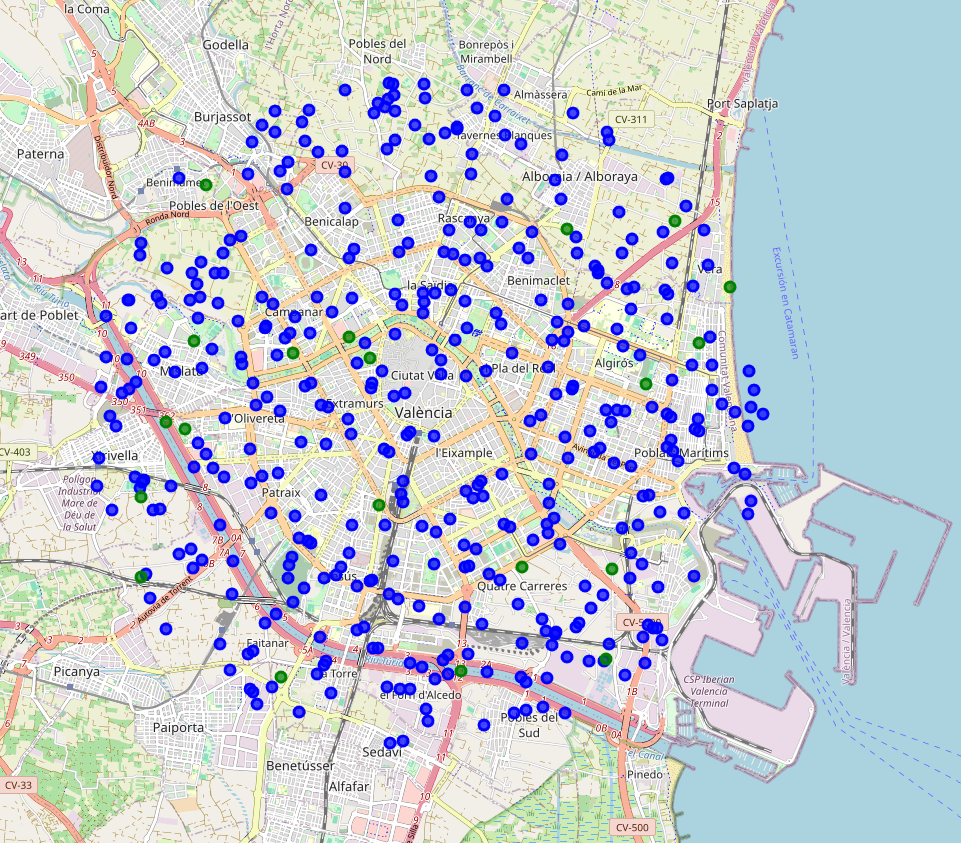
\includegraphics[width=\textwidth]{images/ejemplo_centros_medicos.png}
        \label{fig:poblacion_centros_medicos}
    \end{minipage}
    \hfill
    \begin{minipage}[c]{0.45\textwidth}

        Se representa con 400 puntos azules a la población de la ciudad y alrededores de Valencia. También con 20 puntos verdes las posibles localizaciones de los centros médicos.
    \end{minipage}
    \caption{Población y centros médicos}
\end{figure}

\begin{figure}[H]
    \centering
    \begin{minipage}[c]{0.45\textwidth}
        Ejemplo de solución aleatoria, escogiendo únicamente 5 centros médicos. Podemos ver que al escogerse por el sur y oeste, queda gran parte de valencia con una importante dificultad de acceso a los mismos.
    \end{minipage}
    \hfill
    \begin{minipage}[c]{0.45\textwidth}
        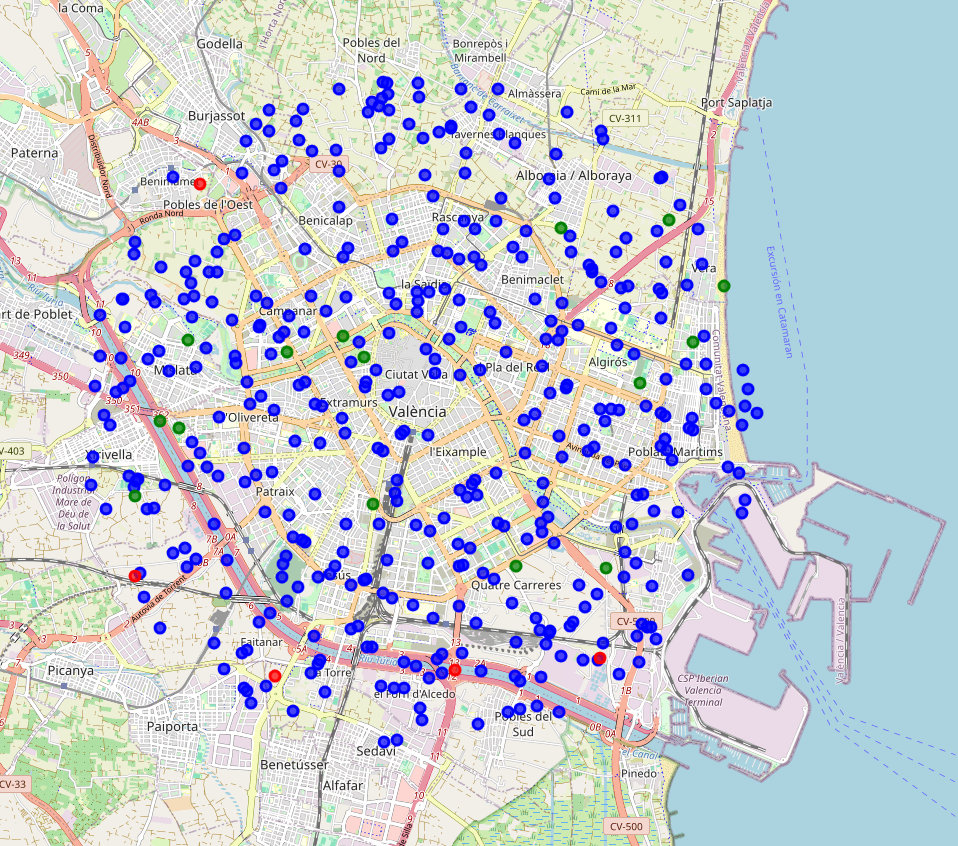
\includegraphics[width=\textwidth]{images/solucion_ejemplo_1.png}
        \label{fig:ejemplo_1}
    \end{minipage}
    \caption{Primer ejemplo de solución}
\end{figure}

\begin{figure}[H]
    \centering
    \begin{minipage}[c]{0.45\textwidth}
        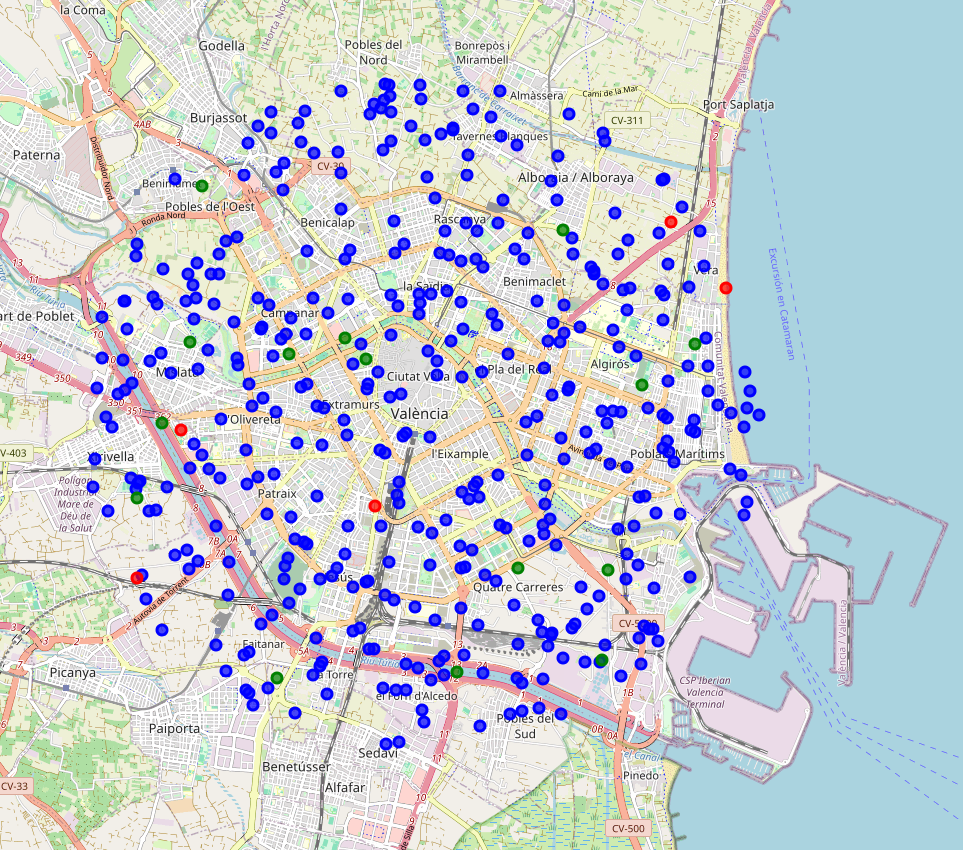
\includegraphics[width=\textwidth]{images/solucion_ejemplo_2.png}
        \label{fig:ejemplo_2}
    \end{minipage}
    \hfill
    \begin{minipage}[c]{0.45\textwidth}
        Aquí ya se pueden ver mejoras, pero sigue sin ser una buena solución. Por el sur y el norte tienen aún bastante lejos los centros médicos, y hay alguno como el de la izquierda del todo, por Valencia Sud, que se utilizará relativamente poco al ir la población a los otros 2 más centricos (estos a su vez quedarán sobre saturados).
    \end{minipage}
    \caption{Segundo ejemplo de solución}
\end{figure}

\begin{figure}[H]
    \centering
    \begin{minipage}[c]{0.45\textwidth}
        Esta solución sería, de las 3, la que mejor apariencia tiene, con una dispersión de los centros médicos mejor, y solo dejando más apartada la zona sur del puerto.
    \end{minipage}
    \hfill
    \begin{minipage}[c]{0.45\textwidth}
        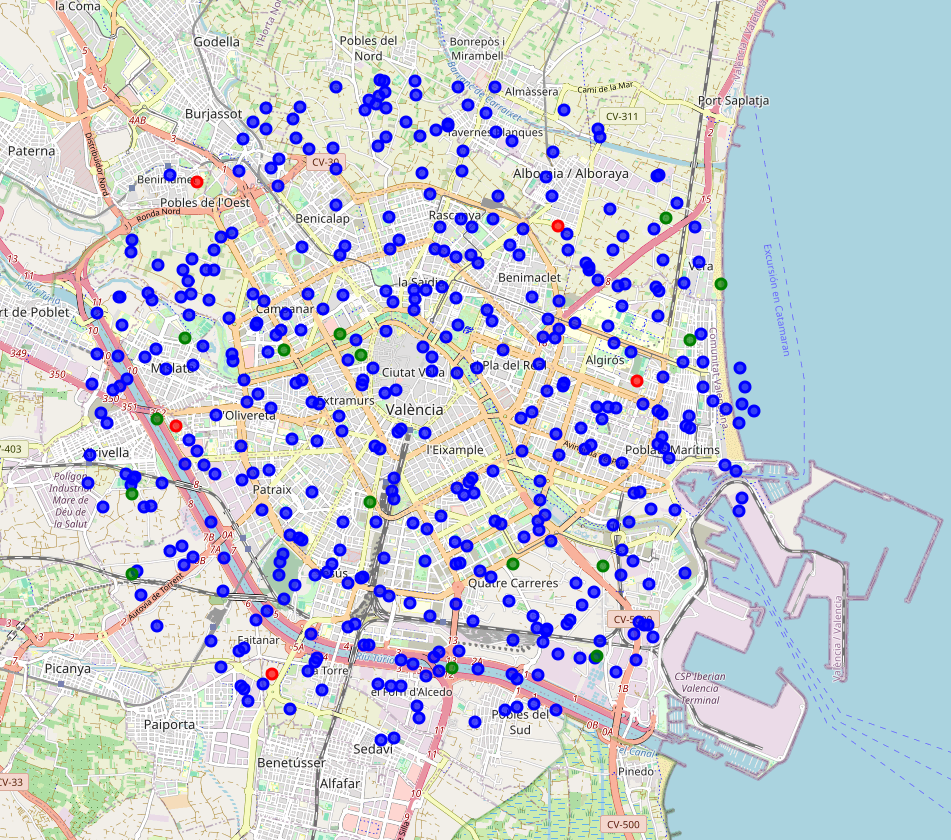
\includegraphics[width=\textwidth]{images/solucion_ejemplo_3.png}
        \label{fig:ejemplo_3}
    \end{minipage}
    \caption{Tercer ejemplo de solución}
\end{figure}

 Con este ejemplo, aunque muy simplificado, seguiría sin ser factible buscar la mejor solución probando combinaciones
 o con un algoritmo exacto.Por ello, he modelizado el problema y usaré una metaheurística GRASP para encontrar soluciones eficientes.\\
 La efectividad de este enfoque se validará comparando los resultados con los publicados en un artículo de referencia que utiliza el mismo conjunto de datos.

\section{Modelo Matemático}
- El modelo no es lineal
- Las variables son discretas
Es multiobjetivo (definir las 3 funciones objetivo)
Definir las restricciones

Explicación de por qué no se puede utilizar un método exacto (optimización no lineal, variables no continuas, espacio no convexo, problema combinatorio)



\chapter{GRASP}
\section{Por qué el GRASP}
- Es un método sencillo de implementar, pero complicado de adaptar para realizar un buen desempeño
- Suele obtener buenas soluciones muy rápido, al contrario que Tabu o Algoritmos Genéticos
- Es especialmente bueno para problemas combinatorios, ya que las búsquedas locales son más fáciles de definir

\section{Metaheurísticas del grasp}
definir primero la monoobjetivo, cómo se comporta, y por qué en monoobjetivo es muy sencillo definir grasp
definir la multiobjetivo, explicar las diferencias que hay con respecto a la búsqueda de soluciones, y los tipos de búsquedas locales que se pueden hacer (por pesos, mejorando las variables por separado ETC)

\section{Implementación del grasp}
Primera versión, grasp con inicialización greedy randomizada (con alpha fijo) y 2 búsquedas locales (aleatorizadas) en serie.

Explicar por qué voy a utilizar aprendizaje reforzado para mejorar el algoritmo

Segunda y última versión, grasp con inicialización greedy randomizada (con alpha ranodom), búsquedas locales escogidas por aprendizaje reforzado.

Explicar la paralelización, como afecta a los pesos del reforzado y a la generación de los frentes de pareto, y cómo mejora la velocidad del algoritmo

\chapter{Experimentación y Resultados}facilita
instancias de ejemplo (2 o 3)

Ajuste de los parámetros del algoritmo (tanto la alpha del greedy como la betha, temperatura y learning rate de la parte de aprendizaje reforzado)

Comparativa entre utilizar o no aprendizaje reforzado (resultados vs tiempos), ya que el reforzado irá mejor, pero será algo más lento (no mucho)

Ahora del algoritmo con aprendizaje reforzado, comparativa con el algoritmo del artículo (greedy con path relinking)

Si se puede encontrar, comparar con los tiempos. Si no, solo comparar el frente de pareto encontrado por x iteraciones del algoritmo vs el frente de pareto del artículo.

Si tengo tiempo, me gustaría implementar el algoritmo en un caso real. Si no, al caso de ejemplo de la ciudad de valencia introducido en el capítulo del modelo matemático

\chapter{Conclusiones}

- El algoritmo va peor, igual, mejora o va distinto 

\chapter{Agradecimientos}
Valgrai, compañeros del máster, amigos, familia, mi tutora del TFM


\begin{thebibliography}{X}
    \bibitem{k-Balanced} \textsc{Sánchez-Oro, Jesús; López-Sánchez, Ana D.; Martínez-Gavara, Anna; Hernández-Díaz, Alfredo G.; Duarte, Abraham}. \textit{A Hybrid Strategic Oscillation with Path Relinking Algorithm for the Multiobjective k-Balanced Center Location Problem.} Mathematics, Vol. 9, No. 8, 2021, Artículo 853. \url{https://www.mdpi.com/2227-7390/9/8/853}

    \bibitem{Numerical_optimization_nocedal_wright}
    Jorge Nocedal and Stephen J. Wright.
    \newblock {\em Numerical Optimization}.
    \newblock Springer, 2nd edition, 2006.

    \bibitem{Dantzig1951} \textsc{Dantzig, George B.} \textit{Maximization of a Linear Function of Variables Subject to Linear Inequalities.} En: Koopmans, Tjalling C. (ed.). \textit{Activity Analysis of Production and Allocation}. New York: John Wiley \& Sons, Inc., 1951, pp. 339-347. \url{https://wwwf.imperial.ac.uk/~ajacquie/IC_Num_Methods/IC_Num_Methods_Docs/Literature/Dantzig2.pdf}

    \bibitem{Bre2017}
    Facundo Bre and Víctor Fachinotti.
    \newblock A computational multi-objective optimization method to improve energy efficiency and thermal comfort in dwellings.
    \newblock {\em Energy and Buildings}, 154: (missing pages, if available), August 2017.
    \newblock \href{https://doi.org/10.1016/j.enbuild.2017.08.002}{DOI: 10.1016/j.enbuild.2017.08.002}
    

\end{thebibliography}


\end{document}

